\hypertarget{ux751fux6210ux6a21ux578b}{%
\chapter{生成模型}\label{ux751fux6210ux6a21ux578b}}

\hypertarget{ux751fux6210ux5bf9ux6297ux7f51ux7edcgans}{%
\section{生成对抗网络（GANs）}\label{ux751fux6210ux5bf9ux6297ux7f51ux7edcgans}}

\hypertarget{ux4e00ux6838ux5fc3ux601dux60f3-2}{%
\subsection{一、核心思想}\label{ux4e00ux6838ux5fc3ux601dux60f3-2}}

生成对抗网络是一个非常巧妙且强大的无监督学习框架，由 Ian Goodfellow 在 2014 年提出。GANs的核心思想是设置一个``二人游戏''。想象一下，我们有两个相互竞争的神经网络：

生成器 (Generator, G)：它的工作是``凭空''创造出看起来很真实的数据（比如，假的毕Z加索画作）。它试图模仿真实数据的分布。

判别器 (Discriminator, D)：它的工作是当一个``鉴定专家''，判断一个输入数据是来自真实数据集（真实的毕加索画作）还是生成器伪造的（假的画作）。

它们通过一种``对抗''的方式共同进化：生成器G努力地学习，试图生成越来越逼真的数据来``欺骗''判别器D；判别器D努力地学习，试图提高自己的鉴别能力，准确``识破''所有来自G的伪造品。这个过程就像一场军备竞赛，最终的理想状态是：生成器G变得非常出色，它造出的``假货''足以以假乱真，后续会证明，这将导致判别器D无法分辨，只能靠猜（即判断为真的概率为 50\%）。

\hypertarget{ux4e8cux76eeux6807ux51fdux6570}{%
\subsection{二、目标函数}\label{ux4e8cux76eeux6807ux51fdux6570}}

\[
\min_G \max_D V(D, G)=\mathbb{E}_{x\sim p_{data}(x)}[\log D(x)] + \mathbb{E}_{z\sim p_z(z)}[\log(1 - D(G(z)))]
\]

\begin{enumerate}
\def\labelenumi{\arabic{enumi}.}
\tightlist
\item
  符号与参与者（The Players）
\end{enumerate}

\begin{itemize}
\tightlist
\item
  \(G\)（生成器）：我们的``伪造者''。它是一个神经网络。
\item
  \(D\)（判别器）：我们的``鉴定专家''。它也是一个神经网络。
\item
  \(x\)：代表一个真实数据（比如一张真实的猫的照片）。
\item
  \(p_{data}(x)\)：真实数据的概率分布（理论上所有真实猫的照片的集合）。\(x \sim p_{data}(x)\) 意味着 \(x\) 是从这个真实数据集中随机抽取的一个样本。
\item
  \(z\)：一个随机噪声向量（通常是从一个简单分布，如高斯分布或均匀分布中采样）。\(z\) 是 \(G\) 创造``灵感''的来源。
\item
  \(p_z(z)\)：噪声向量 \(z\) 的分布。\(z \sim p_z(z)\) 意味着 \(z\) 是从这个噪声分布中随机抽取的一个样本。
\end{itemize}

\begin{enumerate}
\def\labelenumi{\arabic{enumi}.}
\setcounter{enumi}{1}
\tightlist
\item
  网络的输入与输出
\end{enumerate}

\begin{itemize}
\tightlist
\item
  \(G(z)\)：

  \begin{itemize}
  \tightlist
  \item
    输入：噪声 \(z\)。
  \item
    输出：一个``伪造''的数据。\(G\) 试图让 \(G(z)\) 看起来和 \(x\) 一样真实。
  \end{itemize}
\item
  \(D(x)\)：

  \begin{itemize}
  \tightlist
  \item
    输入：一个数据（可能是真实的 \(x\)，也可能是伪造的 \(G(z)\)）。
  \item
    输出：一个介于 0 和 1 之间的概率值。这个值表示 \(D\) 认为这个输入数据是真实的概率。
  \item
    \(D(x)\to 1\) 表示 \(D\) 认为 \(x\) 非常可能是真实的。
  \item
    \(D(x)\to 0\) 表示 \(D\) 认为 \(x\) 非常可能是伪造的。
    这里需要说明的是，对于数据 \(x\)，\(D(x)\) 的真实值服从 0-1 分布，但 \(x\) 的概率分布并不是 0-1 分布。这里运用交叉熵损失时，函数里对应的概率分布应该是 \(D(x)\) 的分布，而不是 \(p_{data}(x)\) 这个 \(x\) 的分布。
  \end{itemize}
\end{itemize}

\(p_{data}(x)\) 则是 \(x\) 本身的概率密度分布，它往往不一定是离散的 \(p(x=\cdots)=\cdots\) 形式，而更可能是一个理论上的、隐式的、未知的概率密度分布，是我们试图用模型去学习和模拟的``目标分布''。比如，想象宇宙中存在一个理想的、完美的函数 \(p_{data}\)，它是所有图片的概率密度函数。如果你给这个函数输入一张非常逼真的、自然的人脸图片，它会输出一个高概率密度 \(0.0001\)；输入一张很怪异的图片，它会输出一个较低的概率值 \(10^{-20}\)。这个 \(p_{data}(x)\) 理论上包含了研究范围内所有``有效''数据（例如所有人脸）的生成规律。

我们虽然没有 \(p_{data}\) 概率密度函数本身，但我们有从这个函数中采样 (Sample) 得到的结果。这个``采样结果''就是你的``训练数据集''，例如，ImageNet 数据集就是 \(p_{data}(x)\)（其中 \(x\) 是``自然图像''）的一组样本。在 GAN 的目标函数中，当看到 \(\mathbb{E}_{x\sim p_{data}(x)}\) 这一项时，它的实际操作含义是：``从你的训练数据集中随机抽取一个 batch 的数据 \(x\)。''我们使用这个经验分布近似 \(p_{data}\)，而随着 GAN 的训练，所谓``逼真''其实就代表 \(G\) 生成的数据（图像）的分布越来越接近给定数据集中的分布。事实上，我们也就认为这是在用端到端的方法近似非常复杂的 \(p_{data}\) 函数。之所以需要 GAN 这样的生成模型，正是因为 \(p_{data}(x)\) 过于复杂，我们无法用传统方法（如最大似然估计）直接对其进行建模，因此只能通过这种``博弈''的方式来间接学习它。

\begin{enumerate}
\def\labelenumi{\arabic{enumi}.}
\setcounter{enumi}{2}
\tightlist
\item
  目标函数的逐项解析
\end{enumerate}

现在我们来看这个函数的两大部分：

\[
V(D,G)=\mathbb{E}_{x\sim p_{data}(x)}[\log D(x)] + \mathbb{E}_{z\sim p_z(z)}[\log(1-D(G(z)))]
\]

\begin{itemize}
\tightlist
\item
  第一项：\(\mathbb{E}_{x\sim p_{data}(x)}[\log D(x)]\)

  \begin{itemize}
  \tightlist
  \item
    含义：这一项衡量的是判别器 \(D\) 正确识别真实数据的能力。
  \item
    \(D\) 的目标（\(\max_D\)）：\(D\) 想要最大化这一项。

    \begin{itemize}
    \tightlist
    \item
      当输入一个真实数据 \(x\) 时，\(D\) 希望自己的输出 \(D(x)\) 尽可能接近 1（即``我确定这是真的''）。
    \item
      当 \(D(x)\to 1\) 时，\(\log D(x)\) 会接近 \(\log(1)=0\)。这是 \(\log\) 函数在其定义域（0 到 1）内的最大值。
    \end{itemize}
  \item
    \(G\) 的目标：\(G\) 对这一项没有控制权，因为它只和真实数据 \(x\) 有关。
  \end{itemize}
\item
  第二项：\(\mathbb{E}_{z\sim p_z(z)}[\log(1-D(G(z)))]\)

  \begin{itemize}
  \tightlist
  \item
    含义：这一项衡量的是判别器 \(D\) 正确识别伪造数据的能力。
  \item
    \(D(G(z))\)：这是 \(D\) 对 \(G\) 生成的假数据 \(G(z)\) 的判断（它认为 \(G(z)\) 是真实的概率）。
  \item
    \(1-D(G(z))\)：这就表示 \(D\) 认为 \(G(z)\) 是伪造的概率。
  \item
    \(D\) 的目标（\(\max_D\)）：\(D\) 想要最大化这一项。

    \begin{itemize}
    \tightlist
    \item
      当输入一个伪造数据 \(G(z)\) 时，\(D\) 希望自己的输出 \(D(G(z))\) 尽可能接近 0（即``我确定这是假的''）。
    \item
      当 \(D(G(z))\to 0\) 时，\(1-D(G(z))\) 接近 1，因此 \(\log(1-D(G(z)))\) 接近 \(\log(1)=0\)。
    \item
      所以，通过让 \(\log D(x)\) 和 \(\log(1-D(G(z)))\) 都趋近于 0，\(D\) 就在最大化 \(V(D,G)\)。
    \end{itemize}
  \item
    \(G\) 的目标（\(\min_G\)）：\(G\) 想要最小化这一项（因为 \(G\) 无法影响第一项）。

    \begin{itemize}
    \tightlist
    \item
      \(G\) 的目标是``欺骗'' \(D\)。它希望 \(D\) 在看到 \(G(z)\) 时，误以为它是真的，即 \(D(G(z))\) 尽可能接近 1。
    \item
      当 \(D(G(z))\to 1\) 时，\(1-D(G(z))\) 接近 0。
    \item
      \(\log(1-D(G(z)))\) 会趋近于 \(\log(0)=-\infty\)。
    \item
      这样，\(G\) 就成功地最小化了 \(V(D,G)\)。
    \end{itemize}
  \end{itemize}
\end{itemize}

\begin{enumerate}
\def\labelenumi{\arabic{enumi}.}
\setcounter{enumi}{3}
\tightlist
\item
  总结：\(\min_G \max_D V(D,G)\)
\end{enumerate}

\begin{itemize}
\tightlist
\item
  \(\max_D V(D,G)\)（判别器的目标）：\(D\) 试图最大化 \(V(D,G)\)。它通过训练，力求做到：

  \begin{enumerate}
  \def\labelenumi{\arabic{enumi}.}
  \tightlist
  \item
    看到真实数据 \(x\)，输出 \(D(x)=1\)。
  \item
    看到伪造数据 \(G(z)\)，输出 \(D(G(z))=0\)。如果 \(D\) 是一个完美的判别器，\(V(D,G)\) 的最大值是 \(0+0=0\)。
  \end{enumerate}
\item
  \(\min_G V(D,G)\)（生成器的目标）：\(G\) 试图最小化 \(V(D,G)\)。它通过训练，力求做到：

  \begin{enumerate}
  \def\labelenumi{\arabic{enumi}.}
  \tightlist
  \item
    生成 \(G(z)\)，让 \(D\) 误判，使得 \(D(G(z))=1\)。当 \(G\) 变得更强时，第二项 \(\log(1-D(G(z)))\) 会被推向 \(-\infty\)。
  \end{enumerate}
\end{itemize}

\begin{enumerate}
\def\labelenumi{\arabic{enumi}.}
\setcounter{enumi}{4}
\tightlist
\item
  目标函数相关拓展
\end{enumerate}

（1）判别器D的目标函数

注意到，这个目标函数 \(V(D, G)\) 的形式与二元交叉熵损失 (Binary Cross-Entropy Loss) 非常相似。把 \(D\) 看作一个二元分类器，真实数据 \((x)\) 的标签为 \(y=1\)；伪造数据 \((G(z))\) 的标签为 \(y=0\)。\(D\) 的目标是最小化分类的交叉熵损失，这等价于最大化我们上面的 \(V(D, G)\)。

\begin{enumerate}
\def\labelenumi{\arabic{enumi}.}
\tightlist
\item
  标准的二元交叉熵（BCE）损失
\end{enumerate}

首先，我们回忆一下标准的二元交叉熵损失函数。它通常用于二元分类问题（比如判断``是''或``否''）。

假设：

\begin{itemize}
\tightlist
\item
  \(y\) 是真实标签（\(y=1\) 表示``真''，\(y=0\) 表示``假''）。
\item
  \(p\) 是你的模型预测 \(y=1\) 的概率。
\end{itemize}

那么，单个样本的 BCE 损失 \(L\) 是：

\[
L(y,p) = -[y\cdot\log(p) + (1-y)\cdot\log(1-p)]
\]

这个公式的含义是：

\begin{itemize}
\tightlist
\item
  如果 \(y=1\)（真实标签为``真''）：损失变为 \(L=-[1\cdot\log(p)+0]=-\log(p)\)。

  \begin{itemize}
  \tightlist
  \item
    为了最小化损失 \(L\)，你需要最大化 \(\log(p)\)，也就是让 \(p\to 1\)。
  \end{itemize}
\item
  如果 \(y=0\)（真实标签为``假''）：损失变为 \(L=-[0+1\cdot\log(1-p)]=-\log(1-p)\)。

  \begin{itemize}
  \tightlist
  \item
    为了最小化损失 \(L\)，你需要最大化 \(\log(1-p)\)，也就是让 \(p\to 0\)。
  \end{itemize}
\end{itemize}

这完全符合我们对分类器的期望。

注意：这里我们的损失项要有两部分：一部分鼓励``把真的分入`真'类别''，真实概率分布为：\(p_{data}\) 满足为 1 时代表符合该类别（``为真''），为 0 时不符合。一部分鼓励``把假的分入`假'类别''，真实概率分布为：\(p_z\) 满足为 1 时代表符合该类别（``为假''），为 0 时不符合。

于是，判别器的总损失可以写成：

\[
L_D = L_{real} + L_{fake} = \mathbb{E}[-\log D(x)] + \mathbb{E}[-\log(1-D(G(z)))]
\]

\[
L_D = -\Bigl(\mathbb{E}[\log D(x)] + \mathbb{E}[\log(1-D(G(z)))]\Bigr)
\]

（为了简洁，我们暂时省略了期望符号 \(\mathbb{E}\) 外的 \(x\sim p_{data}\) 和 \(z\sim p_z\)）

现在，我们再回头看 GANs 的目标函数 \(V(D,G)\)：

\[
V(D,G)=\mathbb{E}[\log D(x)] + \mathbb{E}[\log(1-D(G(z)))]
\]

对比一下 \(L_D\) 和 \(V(D,G)\)，我们能清楚地看到：

\[
V(D,G) = -L_D
\]

（2）生成器G的目标函数

按照原公式，生成器 \(G\) 的目标是最小化 \(\mathbb{E}[\log(1-D(G(z)))]\)。这个目标函数在理论上是完美的，但在实践中，尤其是在训练初期，会引发一个严重的问题：梯度消失 (Vanishing Gradients)。

我们来分析一下为什么：

\begin{enumerate}
\def\labelenumi{\arabic{enumi}.}
\tightlist
\item
  训练初期，\(G\) 很差：一开始，\(G\) 只是一个随机的神经网络，它生成的 \(G(z)\) 都是无意义的噪声（比如一堆雪花点）。
\item
  \(D\) 很容易``碾压'' \(G\)：判别器 \(D\) 的任务很简单：区分``真实的猫''和``一堆雪花点''。\(D\) 会很快学会，并且非常自信地将 \(G\) 生成的 \(G(z)\) 判定为假。
\item
  \(D\) 的输出会发生什么？

  \begin{itemize}
  \tightlist
  \item
    当 \(D\) 看到 \(G(z)\)（雪花点）时，它会非常确定这是假的。
  \item
    因此，\(D(G(z))\) 的输出会非常接近 0。
  \end{itemize}
\item
  \(G\) 的损失函数出了什么问题？

  \begin{itemize}
  \tightlist
  \item
    \(G\) 的损失是 \(L_G=\log(1-D(G(z)))\)。
  \item
    如果 \(D(G(z))\) 接近 0（比如 0.001），\(L_G\) 就会是 \(\log(1-0.001)\approx \log(1)=0\)。
  \item
    这看起来 \(G\) 的损失很``低''（接近 0），但这只是一个假象。真正的问题在于梯度。
  \end{itemize}
\end{enumerate}

让我们看一下 \(G\) 的损失函数 \(L_G=\log(1-p)\) 的图像，其中 \(p=D(G(z))\) 是 \(D\) 的输出：

\begin{itemize}
\tightlist
\item
  X 轴：\(D\) 的输出 \(p\)（从 0 到 1）
\item
  Y 轴：\(G\) 的损失 \(L_G\)
\end{itemize}

注意到：

\begin{itemize}
\tightlist
\item
  当 \(p\) 接近 0 时（也就是 \(D\) 非常自信地判定 \(G(z)\) 为假时），这条曲线非常平坦。
\item
  ``平坦''在微积分中意味着斜率（梯度）接近 0。
\end{itemize}

这就是灾难发生的地方：\(G\) 生成了很差的图像 \(\rightarrow\) \(D\) 自信地将其判为假（\(p\approx 0\)）\(\rightarrow\) \(G\) 得到的损失函数梯度 \(\approx 0\) \(\rightarrow\) \(G\) 无法更新参数，它完全学不到东西。

这个问题被称为``饱和'' (Saturating)：\(G\) 在它最需要学习的时候（即它表现最差的时候）反而学得最慢。

原始论文的作者提出了一个简单而实际的修正方法。

他们建议，不要让 \(G\) 最小化 \(\log(1-D(G(z)))\)，而是让 \(G\) 最大化 \(\log(D(G(z)))\)。

\begin{itemize}
\tightlist
\item
  旧损失（蓝色）：\(\log(1-p)\)。当 \(p \rightarrow 0\) 时，梯度是平坦的（消失）。
\item
  新损失（绿色）：\(-\log(p)\)。当 \(p \rightarrow 0\) 时，梯度极其陡峭（趋向 \(-\infty\)）。
\end{itemize}

这个新的损失函数具有我们正想要的特性：它恰好在 \(G\) 表现最差时（即 \(D(G(z))\) 接近 0 时）提供了巨大而强烈的梯度信号。这使得 \(G\) 在训练一开始就能够快速学习。

但此时其实仍然没有完全解决梯度消失问题。

\[
\nabla_{\theta_g} L_G = \nabla_{\theta_g}[-\log(D(G(z)))]
\]

通过链式法则，我们把它分解成三部分：

\[
\nabla_{\theta_g} L_G =
\frac{d(-\log p)}{dp}
\cdot
\nabla_a D(a)\rvert_{a=G(z)}
\cdot
\nabla_{\theta_g} G(z)
\]

其中 \(p=D(G(z))\) 是 \(D\) 的最终输出，\(a=G(z)\) 是 \(D\) 的输入。三部分分别对应：来自 \(G\) 损失的梯度、来自 \(D\) 内部的梯度、来自 \(G\) 内部的梯度。

Part 1：关注的部分

\[
\frac{d(-\log p)}{dp}=-\frac{1}{p}
\]

\begin{itemize}
\tightlist
\item
  当 \(G\) 很差时，\(p=D(G(z)) \rightarrow 0\)。
\item
  这一项 \(-\frac{1}{p}\) 趋向无穷大。
\item
  也就是说，\(G\) 的损失函数本身正在``拼命地''产生一个巨大的信号。
\end{itemize}

Part 2：``真正消失''的部分

\[
\nabla_a D(a)
\]

也就是 \(\nabla_{G(z)}D(G(z))\)，它表示 \(D\) 的输出概率 \(p\) 相对于 \(D\) 的输入 \(a\) 的梯度。\(D\) 如何输出一个 0 到 1 的概率？它的最后一层是一个 Sigmoid 函数。\(D\) 的目标是把真假拉开；当它变得很强时（不重叠），它会给 \(G(z)\) 一个极低的分数。为了输出 \(p \rightarrow 0\)，Sigmoid 函数的输入（logits）必须是一个很大的负数（比如 -10、-20）。

\begin{figure}[htbp]
\centering
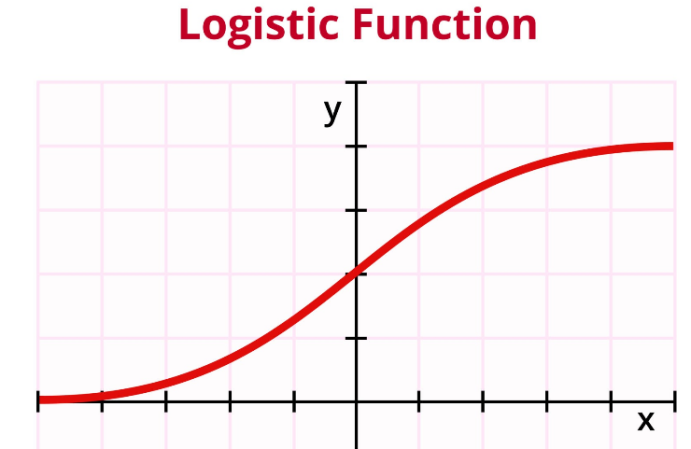
\includegraphics{images/image-0011.png}
\caption{Logistic Function}
\end{figure}

在 \(x\) 很小或很大时，用于把输出转换为概率的 Sigmoid 函数的导数（梯度）趋近于 \(0\)。

\(G\) 的总梯度是：

\[
\nabla_{\theta_g} L_G =
(\mathcjk{趋向无穷大}) \cdot (\mathcjk{趋向 }0) \cdot (\mathcjk{来自 }G\mathcjk{ \mathcjk{的梯度}})
\]

第一项来自 \(\log\)，第二项来自 Sigmoid。
在这个不定型中，Sigmoid函数往往占主导，导致梯度消失。类比就是打开了``消防栓''，但``水管''（D网络）内部被``水垢''（Sigmoid 函数）给堵住了。当D变得很强时，它内部的 Sigmoid 函数会饱和（变得平坦）。这个``平坦''的 Sigmoid 层就像一个被水垢堵住的、极窄的瓶颈（梯度趋于0）。WGAN通过修改D函数，解决了这个问题（见后）。

\hypertarget{ux56dbux8badux7ec3ux7ec8ux70b9}{%
\subsubsection{（四）训练终点}\label{ux56dbux8badux7ec3ux7ec8ux70b9}}

假设我们有一个固定的生成器 \(G\)，我们想找到能最大化 \(V(D,G)\) 的最优判别器 \(D^*\)。

我们的目标函数是：

\[
V(D,G)=\int_x p_{data}(x)\log(D(x))dx+\int_z p_z(z)\log(1-D(G(z)))dz
\]

为了简化，我们知道 \(G(z)\) 会形成一个伪造数据的分布 \(p_g(x)\)，所以我们可以把第二项也写成关于 \(x\) 的积分：

\[
V(D,G)=\int_x [p_{data}(x)\log(D(x))+p_g(x)\log(1-D(x))]dx
\]

要找到使这个积分最大的 \(D(x)\)，我们只需要看积分号里的函数（被积函数），并对任意一个 \(x\) 求它的最大值。

令 \(a=p_{data}(x)\) 和 \(b=p_g(x)\)，我们要找 \(D\) 来最大化 \(f(D)=a\log(D)+b\log(1-D)\)。这是一个标准的求极值问题，我们对 \(D\) 求导并令其为 0：

\[
\frac{df}{dD}=\frac{a}{D}-\frac{b}{1-D}=0
\]

于是：

\[
a=(a+b)D \Rightarrow D=\frac{a}{a+b}
\]

把 \(a\) 和 \(b\) 换回来，我们就得到了最优判别器 \(D^*(x)\)：

\[
D^*(x)=\frac{p_{data}(x)}{p_{data}(x)+p_g(x)}
\]

以上推导通过对D求导，找到了使得V(D,G)最大的D，也就是最优判别器。这个公式告诉我们，一个完美的判别器，其输出概率D(x)应该等于``这个x来自真实数据的概率''除以``它来自真实数据或伪造数据的总概率''。

当然，判别器的训练只是手段，最终训练终点还要看生成器的输出。容易想到，如果 \(G\) 变得完美，伪造数据完全学习了真实数据的分布，\(p_g(x)=p_{data}(x)\)，则 \(D^*(x)=1/2\)。下面我们来严格证明，当判别器 \(D\) 取 \(D^*\) 时，\(\max_D V(D,G)=V(D^*,G)\) 关于 \(G\) 最小等价于取到这种情况。

\[
C(G)=\max_D V(D,G)=V(D^*,G)
\]

\[
C(G)=\mathbb{E}_{x\sim p_{data}}\left[\log\frac{p_{data}}{p_{data}+p_g}\right]
+\mathbb{E}_{x\sim p_g}\left[\log\frac{p_g}{p_{data}+p_g}\right]
\]

注意：这里把 \(p_{data}(x)\) 简写为 \(p_{data}\)，把 \(p_g(x)\) 简写为 \(p_g\)。

经过一点数学变换，这个表达式可以被重写为：

\[
C(G)=2\cdot D_{JSD}(p_{data}\parallel p_g)-2\log 2
\]

\begin{itemize}
\tightlist
\item
  \(D_{JSD}\) 代表 Jensen-Shannon Divergence（JSD，杰森-香农散度）。
\item
  散度（Divergence）是信息论中用来衡量两个概率分布之间差异性的数学工具。
\end{itemize}

\(G\) 的最终目标是 \(\min_G C(G)\)，也就是：

\[
\min_G [2\cdot D_{JSD}(p_{data}\parallel p_g)-2\log 2]
\]

训练生成器 \(G\) 的最终数学目标，就是最小化真实数据分布 \(p_{data}(x)\) 和伪造数据分布 \(p_g(x)\) 之间的 JSD 散度，当且仅当两个分布完全相同时，即 \(p_g(x)=p_{data}(x)\) 时，JSD 散度才为 \(0\)。总之，目标函数中 \(\min_G\) 和 \(\max_D\) 博弈的巧妙设计，使得 \(G\) 的任务变成了学习一个完美的 \(p_g\) 分布，使其与 \(p_{data}\) 一致。

\hypertarget{ux4e09gansux7684ux5e94ux7528}{%
\subsection{三、GANs的应用}\label{ux4e09gansux7684ux5e94ux7528}}

\begin{enumerate}
\def\labelenumi{\arabic{enumi}.}
\tightlist
\item
  图像生成与艺术创作
\end{enumerate}

这是GANs最著名的应用。目标是让模型学习一个庞大数据集（比如10万张人脸照片）的``精髓''，然后能从一个随机噪声向量 \(z\) 出发，生成一张全新的、不属于数据集中任何一张，但又看起来极其逼真的人脸。可以用 StyleGAN、BigGAN 等模型生成不存在的``模特''照片、创造数字艺术、游戏角色设计。

与变分自编码器（Variational Autoencoders, VAEs）相比：

\textbf{GANs}

\begin{itemize}
\tightlist
\item
  核心思想：对抗（Adversarial），一个生成器和一个判别器相互博弈。
\item
  训练目标：欺骗判别器，即 \(G\) 的目标是让 \(D\) 无法区分真假。
\item
  生成质量：高保真（Sharp）。由于 \(D\) 的存在，\(G\) 被迫生成清晰、锐利的图像边缘和纹理，否则很容易被判别为假。
\item
  潜空间 \(z\)：通常较纠缠（Entangled）。原始 GANs 的 \(z\) 空间较无序，改变 \(z\) 的一个维度，可能同时改变人脸的多个特征，如头发、年龄、朝向。
\end{itemize}

\textbf{VAEs}

\begin{itemize}
\tightlist
\item
  核心思想：编码-解码（Encoding-Decoding），编码器将图像压缩成潜空间 \(z\) 中的概率分布，解码器再从 \(z\) 中采样并重建图像。
\item
  训练目标：最小化重建损失，让解码后的图像与原始图像尽可能接近。
\item
  生成质量：较模糊（Blurry）。VAEs 最小化像素级平均误差（如 \(L_2\) 损失），这会鼓励模型生成更``安全''的平均图像。
\item
  潜空间 \(z\)：更平滑（Smooth）。VAEs 的 \(z\) 空间被正则化为连续且平滑的结构，适合在两张人脸的 \(z\) 向量之间做插值。
\end{itemize}

VAEs 擅长学习一个平滑且有意义的潜空间（适合插值和理解数据结构），但生成结果偏模糊。GANs 擅长生成高度逼真的图像（适合追求视觉保真度），但训练更不稳定，潜空间也不如VAEs规整。

\begin{enumerate}
\def\labelenumi{\arabic{enumi}.}
\setcounter{enumi}{1}
\tightlist
\item
  图像到图像的转换
\end{enumerate}

这类应用的目标是：给定一张输入图像 A，将其转换为另一张具有特定风格或特征的输出图像 B。这里，输入和输出都是图像，而且往往在结构上有一定的对应关系。典型模型如 Pix2Pix（需要成对的训练数据，比如一张草图对应一张照片）、CycleGAN（不需要成对数据，通过循环一致性损失实现非配对转换）。应用如将航拍地图转换为谷歌地图样式，将黑白照片上色，将手绘草图转换为逼真照片，将白天场景转换为夜晚场，将物体从语义分割图还原为真实图像等。在这个领域，传统的神经网络架构主要依赖于编码器-解码器（Encoder-Decoder）结构，通常是卷积神经网络（CNNs），并且常常会加入跳跃连接（如 U-Net 结构）来保留细节。

基于 GANs 的方法（如 Pix2Pix、CycleGAN）与基于 CNNs 的编码器-解码器（如 U-Net）相比：

\textbf{基于 GANs 的方法}

\begin{itemize}
\tightlist
\item
  核心思想：学习映射 \(G\) 和判别真假 \(D\)。生成器 \(G\) 学习从 A 域到 B 域的映射，判别器 \(D\) 判断 \(G\) 生成的 B 是否像真实的 B 域图像。
\item
  损失函数：对抗损失加像素级损失。除了让 \(G\) 骗过 \(D\) 的对抗损失外，还会结合 \(L_1\) 或 \(L_2\) 损失，确保生成图像与目标在像素层面相似。
\item
  生成质量：细节更丰富、更真实。判别器 \(D\) 的存在迫使生成器 \(G\) 生成高频细节，使图像在复杂纹理和结构上更逼真、更锐利。
\item
  对数据对的需求：Pix2Pix 需要成对数据；CycleGAN 不需要成对数据，而是通过循环一致性损失学习非配对转换。
\item
  灵活性：高度灵活，可以学习风格迁移、物体转化等非常规映射。CycleGAN 甚至能在没有直接对应样本的情况下进行域转换。
\end{itemize}

\textbf{基于 CNNs 的编码器-解码器}

\begin{itemize}
\tightlist
\item
  核心思想：学习像素级映射。编码器逐步提取特征，解码器逐步重建图像，中间通过跳跃连接传递细节。
\item
  损失函数：通常使用 \(L_1\) 或 \(L_2\) 像素级损失，衡量生成图像和目标图像之间的像素差异。
\item
  生成质量：可能更平滑、更模糊。纯粹的像素级损失（如 \(L_2\)）会倾向于生成像素平均值，导致图像缺乏锐利细节和真实感。
\item
  对数据对的需求：通常需要大量输入 A 与输出 B 的成对数据。
\item
  灵活性：相对受限，主要用于重建、去噪、超分辨率等有明确像素级对应关系的转换。
\end{itemize}

基于 CNNs 的编码器-解码器 方法（如U-Net）在有大量成对数据且任务偏向于结构性恢复（如图像去噪、超分辨率）时表现良好，但可能缺乏真实感。GANs 通过引入判别器，能够生成更具真实感和高频细节的图像，即使在任务更具创意性或缺乏成对数据（如CycleGAN）时也能出色完成。

\begin{enumerate}
\def\labelenumi{\arabic{enumi}.}
\setcounter{enumi}{2}
\tightlist
\item
  数据增强与模拟
\end{enumerate}

有时，我们的真实数据非常少或非常昂贵。如在医学影像（如CT或MRI）中，要诊断一种罕见的癌症。我们可能只有几百张（甚至几十张）带标签的``阳性''图像。如果只用这点数据去训练一个AI模型，它很难学会，而且极易``过拟合''。这时我们往往采取以下方案：

（1）对已有数据进行变换：对于图像而言，就是旋转、裁剪、缩放、翻转、平移、添加噪声、改变对比度或亮度等。

（2）迁移学习：利用预训练模型进行微调。

（3）利用VAE（变分自编码器）：在编码-解码的过程中，一个 VAE 的编码器输出一个概率分布，解码器不是从一个``点''来重建，而是从这个``模糊区域''中随机采样一个点来进行重建。

（4）利用GAN生成：我们可以训练一个基于生成器-判别器架构的GANs模型（比如一个变种的DCGAN或WGAN），判别器以这几百张真实癌症图像的分布为参考基准。一旦训练完成，这个GANs的生成器就可以从随机噪声开始，生成成千上万张看起来逼真、但又与原始图像不完全相同的``假''癌症图像。

这种方法在其他领域也有很多应用。金融中，也可以用其模拟生成逼真的（但非真实的）欺诈交易数据，用于训练反欺诈系统。自动驾驶中，可以生成更多在现实中难以采集的``边缘案例''驾驶场景（如暴风雪中的行人、罕见的交通事故）。

基于 GANs 的数据增强与传统数据增强相比：

\textbf{基于 GANs 的数据增强}

\begin{itemize}
\tightlist
\item
  核心思想：生成新样本（Generation）。模型学习真实数据的潜在分布 \(p_{\mathrm{data}}\)，再从这个分布中采样，创造全新的数据点。
\item
  具体方法：训练一个完整的生成器 \(G\) 来``伪造''数据。
\item
  数据多样性：理论上更高。它能生成原始数据集中不存在、但仍属于同一分布的新组合，例如一个``介于 A 和 B 之间''的新病灶。
\item
  解决的问题：数据稀缺和不平衡。当某一类别的数据（如罕见病）极度稀缺时，GANs 可以补充该类别样本。
\item
  挑战：训练不稳定，容易出现模式崩溃（Mode Collapse），即 \(G\) 只学会生成少数几种``安全''的假样本。
\end{itemize}

\textbf{传统数据增强}

\begin{itemize}
\tightlist
\item
  核心思想：变换旧样本（Transformation）。对已有数据进行简单的几何或颜色变换。
\item
  具体方法：旋转、裁剪、缩放、翻转、平移、添加噪声、改变对比度或亮度。
\item
  数据多样性：相对较低。生成的数据与原始数据高度相关，一张``旋转过的猫''在本质上并没有提供关于``猫''的全新信息。
\item
  解决的问题：缓解过拟合，通过增加训练数据的``表面''数量，使模型看到更多变化，防止它记住特定训练样本。
\item
  挑战：方法简单有效、成本低，但难以创造真正新的类别内变化。
\end{itemize}

\hypertarget{ux53c2ux8003ux6587ux732e-36}{%
\subsection{参考文献}\label{ux53c2ux8003ux6587ux732e-36}}

\begin{itemize}
\tightlist
\item
  Goodfellow, I., Pouget-Abadie, J., Mirza, M., et al.~(2014). \href{https://papers.nips.cc/paper/5423-generative-adversarial-nets}{Generative Adversarial Nets}. NeurIPS 2014.
\end{itemize}

\clearpage

\hypertarget{gansux8badux7ec3ux7684ux6a21ux5f0fux5d29ux6e83ux95eeux9898ux4e0eux89e3ux51b3ux65b9ux6848}{%
\section{GANs训练的模式崩溃问题与解决方案}\label{gansux8badux7ec3ux7684ux6a21ux5f0fux5d29ux6e83ux95eeux9898ux4e0eux89e3ux51b3ux65b9ux6848}}

\hypertarget{ux4e00ux6a21ux5f0fux5d29ux6e83}{%
\subsection{一、模式崩溃}\label{ux4e00ux6a21ux5f0fux5d29ux6e83}}

假设我们正在训练一个 GAN 来生成手写数字（如 MNIST 数据集，包含 0 到 9）。一个成功的 G（生成器）应该能生成所有 10 种不同的、逼真的数字（0, 1, 2, 3, 4, 5, 6, 7, 8, 9）。

如果 \(G\) 和 \(D\) ``对抗实力相同''，并``共同进化''，是不会发生这种情况的。但事实上判别器 \(D\) 在训练早期常学得太快，很快就识别出了 \(G\) 生成的是假的。由于 \(G\) 在各个方向生成得都不好，\(G\) 收到的梯度方向非常混乱，且前面讲述过，\(D\) 函数内部的 Sigmoid 函数会导致 \(p \to 0\) 时梯度消失，这些梯度的幅度比较小。

这时 \(G\) 可能在训练中偶然发现，自己生成的``7''这个数字特别逼真（概率显著大于 \(0\)），每次都能轻易地骗过 \(D\)（判别器）。由于 \(G\) 的唯一目标就是骗过 \(D\)，它会在这一片混乱的梯度中，生成``7''的方向作为唯一稳定的梯度方向，且往往幅度较大。这会把模型引向生成更多``7''的方向，这时便会有更多正反馈，更多梯度让模型进一步导向生成``7''。无论给它什么随机噪声 \(z\) 作为输入，它的输出都是一个（或一小组）看起来差不多的``7''。在这种情况下，我们就说 \(G\) ``崩溃''到了一个单一的模式（数字 ``7''）上，而完全忽略了数据集中的其他所有``模式''（0, 1, 2, 3\ldots）。

\hypertarget{ux4e8cux6a21ux5f0fux5d29ux6e83ux7684ux89e3ux51b3ux65b9ux6848}{%
\subsection{二、模式崩溃的解决方案}\label{ux4e8cux6a21ux5f0fux5d29ux6e83ux7684ux89e3ux51b3ux65b9ux6848}}

\hypertarget{ux4e00wgan}{%
\subsubsection{（一）WGAN}\label{ux4e00wgan}}

WGAN (Wasserstein GAN)，原始 GAN 的``对抗''太激烈了，尤其是判别器 \(D\) 变得太好时，会让生成器 \(G\) 无法学习。为了解决这个问题，WGAN 做了几个关键的改变。

\begin{enumerate}
\def\labelenumi{\arabic{enumi}.}
\tightlist
\item
  改变D的工作和目标函数
\end{enumerate}

原始 GAN 中，\(D\) 是一个分类器 (Classifier)。输出一个 0 到 1 之间的概率（``这是假的'' vs ``这是真的''）；WGAN 中，\(D\) 被重新定义为一个评论家 (Critic)。它不再输出一个概率，而是输出一个分数 (Score)，撤掉了原来的 Sigmoid 函数。这个分数可以（理论上）是任何实数（比如 \(-10, 0, 50\)）。\(D\) 的目标变成了：给真实数据 \(x\) 尽量打高分，给伪造数据 \(G(z)\) 尽量打低分。\(G\) 的目标也随之改变：努力生成 \(G(z)\)，让 \(D\) 给它打出尽可能高的分。

\begin{enumerate}
\def\labelenumi{\arabic{enumi}.}
\setcounter{enumi}{1}
\tightlist
\item
  梯度正则化
\end{enumerate}

\(D\) 的目标变成了给真实数据 \(x\) 尽量打高分，给伪造数据 \(G(z)\) 尽量打低分，但如果一味鼓励拉开高低分，会让 \(D\) 为了拉开高低分而让自己的打分曲线变得``过于陡峭''，导致梯度爆炸。原始方法是权重裁剪 (Weight Clipping)，这是 WGAN 原始论文中提出的方法，强行检查它的每一个权重，如果某个权重超过了一个小范围（比如 \(0.01\)），就把它强行``拉回''到 \(0.01\)；如果低于 \(-0.01\)，就把它``拉回''到 \(-0.01\)。这会导致逐层梯度相乘过程中发生梯度消失 (Vanishing Gradients)，且表达能力受限 (Limited Capacity)：\(D\) 为了满足这个约束，会``偷懒''，把大部分权重都推到边界值（\(0.01\) 或 \(-0.01\)），变成了一个非常简单的函数，只能用``好''或``坏''等词来打分，失去了学习复杂、精细打分曲线的能力。

于是我们选择用如下数学公式作为惩罚项：

\[
\lambda \cdot (\lVert \nabla D(x) \rVert - 1)^2
\]

这就迫使 \(D\) 在训练中必须时时刻刻调整自己的打分曲线，使其在任何地方的``坡度''都尽量保持在 \(1\) 左右。考虑到实际计算开销，我们一般选取真实与伪造的中间点计算惩罚项：

\begin{enumerate}
\def\labelenumi{\arabic{enumi}.}
\item
  取样：我们从数据集中随机取一个真实图像 \(x_{real}\)。
\item
  生成：我们让 \(G\) 生成一个伪造图像 \(x_{fake}\)。
\item
  插值：我们在这两个图像之间随机选择一个``中间点'' \(\hat{x}\)（读作 x-hat）。

  在数学上，我们随机选一个 0 到 1 之间的小数 \(\epsilon\)，然后计算 \(\hat{x}=\epsilon\cdot x_{real}+(1-\epsilon)\cdot x_{fake}\)。这就像在两个点的连线上随机找一个点。
\item
  检查：我们只在这个``中间点'' \(\hat{x}\) 上计算梯度惩罚：
\end{enumerate}

\[
(\lVert \nabla D(\hat{x}) \rVert - 1)^2
\]

为什么这个``中间点''策略有效？想象 \(D\) 的``打分地貌''。我们强迫 \(D\) 在``真实国度''和``伪造国度''之间的整个广阔地带，都必须保持一个平滑的、坡度为 \(1\) 的``山坡''。这使得 \(G\) 无论身处``伪造国度''的哪个角落，都能清晰地看到一条通往``真实国度''的、坡度恒定的上山路径。而在这样的情况下，这个函数在``真实国度''与``伪造国度''的内部梯度极大概率也接近 \(1\)。

\begin{enumerate}
\def\labelenumi{\arabic{enumi}.}
\setcounter{enumi}{2}
\tightlist
\item
  训练终点
\end{enumerate}

我们之前在讨论 GANs 的目标函数时，推导出过这个结论：对于一个固定的 \(G\)，能让 \(V(D,G)\) 最大的那个``最优'' \(D^*\) 是：

\[
D^*(x)=\frac{p_{data}(x)}{p_{data}(x)+p_g(x)}
\]

当 \(G\) 试图最小化 \(\max_D V(D,G)\) 时，它实际上是在最小化 \(C(G)\)：

\[
C(G)=2\cdot JSD(p_{data}\parallel p_g)-2\log 2
\]

所以，\(G\) 的目标（最小化 \(C(G)\)）等价于最小化 \(p_{data}\) 和 \(p_g\) 之间的 JSD 散度。

当 \(p_{data}\) 和 \(p_g\) 完全不重叠时，JSD 会卡在恒定的最大值（\(\log 2\)），其梯度变为 \(0\)。证明：

KL 散度 \(D_{KL}(P\parallel Q)\) 衡量从分布 \(P\) 切换到分布 \(Q\) 时``损失''了多少信息：

\[
D_{KL}(P\parallel Q)=\sum_x P(x)\log\left(\frac{P(x)}{Q(x)}\right)
\]

JSD 散度只是 KL 散度的一个``平滑、对称''版本。首先定义一个``平均分布''：

\[
M=\frac{1}{2}(p_{data}+p_g)
\]

然后：

\[
JSD(p_{data}\parallel p_g)=\frac{1}{2}D_{KL}(p_{data}\parallel M)+\frac{1}{2}D_{KL}(p_g\parallel M)
\]

在``不重叠''的情况下，先看 \(D_{KL}(p_{data}\parallel M)\)：

\[
D_{KL}(p_{data}\parallel M)=\sum_x p_{data}(x)\log\left(\frac{p_{data}(x)}{M(x)}\right)
\]

把 \(M(x)=\frac{1}{2}(p_{data}(x)+p_g(x))\) 代入：

\[
D_{KL}(p_{data}\parallel M)=\sum_x p_{data}(x)\log\left(\frac{p_{data}(x)}{\frac{1}{2}(p_{data}(x)+p_g(x))}\right)
\]

现在，我们只看那些 \(p_{data}(x)>0\) 的点；因为在其他地方 \(p_{data}(x)=0\)，整个求和项都为 0。

在这些点上，由于 \(p_{data}(x)>0\) 且 \(p_g(x)=0\)，所以：

\[
\frac{p_{data}(x)}{\frac{1}{2}(p_{data}(x)+p_g(x))}=2
\]

因此：

\[
D_{KL}(p_{data}\parallel M)=\sum_x p_{data}(x)\log 2=\log 2
\]

同理，\(D_{KL}(p_g\parallel M)=\log 2\)，所以 \(JSD(p_{data}\parallel p_g)=\log 2\)，变成了常数。故 \(C(G)\) 这时为常数，对 \(G\) 的梯度为 0，也就无法驱动生成器 \(G\) 的参数改变。

\hypertarget{ux4e8cux566aux58f0ux6ce8ux5165}{%
\subsubsection{（二）噪声注入}\label{ux4e8cux566aux58f0ux6ce8ux5165}}

``噪声注入'' (Noise Injection) 的原理，就是用来``对抗'' \(G\)（生成器）变得``太确定''、``太死板''的。``模式崩溃''的发生是因为 \(G\) 找到了一个``捷径''：它发现只要生成``7''这个数字，\(D\)（判别器）就没法分辨。于是 \(G\) 就``偷懒''了，无论给它什么输入 \(z\)，它都只生成``7''。从而我们还在``生产线''的中间好几个工序（即 \(G\) 的中间层）上，随机``洒''上一些新的、小的噪声。

它让 \(D\) 的``记忆''失效了。没有抖动时 \(D\) 可能会学会``记住'' \(G\) 生成的那个``完美的7''。它只要看到这个``完美的7''，就给出某个特定的置信度分数。加入噪声后，即使 \(G\) 两次都想生成那个``完美的7''，但由于``抖动''的存在，它两次生成的``7''都会有细微的、随机的差别。\(D\) 被迫去学习数字真正的、普遍的特征（比如它该有的笔画、结构），而不是去记 \(G\) 的某一个``作品''。这反过来又``逼迫'' \(G\) 必须学会生成各种各样、符合模式的、高质量的数字，而不能只依赖一个``捷径''。通过在中间层增加随机性，迫使 \(G\) 学习一个更健壮、更多样化的``生成策略''，从而防止它``崩溃''到一个单一的模式上。

\hypertarget{ux53c2ux8003ux6587ux732e-37}{%
\subsection{参考文献}\label{ux53c2ux8003ux6587ux732e-37}}

\begin{itemize}
\tightlist
\item
  Goodfellow, I., Pouget-Abadie, J., Mirza, M., et al.~(2014). \href{https://papers.nips.cc/paper/5423-generative-adversarial-nets}{Generative Adversarial Nets}. NeurIPS 2014.
\item
  Arjovsky, M., Chintala, S., \& Bottou, L. (2017). \href{https://arxiv.org/abs/1701.07875}{Wasserstein GAN}. ICML 2017.
\end{itemize}

\clearpage

\hypertarget{ux53d8ux5206ux81eaux7f16ux7801ux5668vaeux4e0evq-vae}{%
\section{变分自编码器（VAE）与VQ-VAE}\label{ux53d8ux5206ux81eaux7f16ux7801ux5668vaeux4e0evq-vae}}

\hypertarget{ux4e00vaeux53d8ux5206ux81eaux7f16ux7801ux5668}{%
\subsection{一、VAE（变分自编码器）}\label{ux4e00vaeux53d8ux5206ux81eaux7f16ux7801ux5668}}

\hypertarget{ux4e00ux6838ux5fc3ux601dux60f3ux548cux67b6ux6784}{%
\subsubsection{（一）核心思想和架构}\label{ux4e00ux6838ux5fc3ux601dux60f3ux548cux67b6ux6784}}

\begin{enumerate}
\def\labelenumi{\arabic{enumi}.}
\tightlist
\item
  核心思想：从``确定''到``概率''
\end{enumerate}

传统自编码器的问题：它的编码器直接将输入数据压缩为一个固定的、确定性的潜向量。当你想生成新数据时，从这个潜空间中随机采样一个点，解码出的结果很可能是无意义的噪声，因为你无法保证这个随机点位于模型学习到的数据流形上。

VAE的解决方案：VAE的编码器不再输出一个单一的向量，而是输出一个概率分布，通常是一个高斯分布，由均值（μ）和方差（σ²）两个向量来描述。这意味着对于每一个输入，模型学习的是它在潜空间中的一个可能区域，而不是一个确切点。

根据任务需要，我们可以只取VAE的编码器，或者把编码器和解码器合起来。由于前面所述，解码器需要在概率空间中采样，因此输出不可能与输入完全相同，但输出的统计学分布却会和输入一致。因此把编码器和解码器合起来实际上是一个``模仿器''，它会输出一批和输入分布相同的新数据（因而可用于数据增强等）。

\begin{enumerate}
\def\labelenumi{\arabic{enumi}.}
\setcounter{enumi}{1}
\tightlist
\item
  关键机制：如何学习这个分布？
\end{enumerate}

编码：输入数据~x，编码器输出潜空间中对应的分布参数~μ~和~log(σ²)。

采样：从这个分布~N(μ, σ²)~中随机采样一个潜向量~z。这个步骤是关键的，因为它允许梯度在训练时通过这个随机操作反向传播（通过重参数化技巧）。

解码：将采样的潜向量~z~送入解码器，尝试重建出原始输入~x'。

\begin{enumerate}
\def\labelenumi{\arabic{enumi}.}
\setcounter{enumi}{2}
\tightlist
\item
  损失函数：双重目标
\end{enumerate}

VAE的损失函数由两部分组成，完美体现了其设计思想：

重构损失：衡量解码器输出的重建数据~x'~与原始输入~x~的差异（如均方误差或交叉熵）。这确保了编码后的信息能够有效地还原数据。

KL散度损失：衡量编码器输出的分布~N(μ, σ²)~与先验分布（通常是标准正态分布~N(0, 1)）之间的差异。这个损失项起到了正则化的作用：

它迫使所有编码后的分布都向原点附近聚集，让潜空间变得连续、平滑且有结构。

它避免了编码器``作弊''，比如为每个输入学习一个方差为0的分布（退化成确定性编码），或者把不同的输入编码到相距甚远的区域。

\begin{enumerate}
\def\labelenumi{\arabic{enumi}.}
\setcounter{enumi}{3}
\tightlist
\item
  优势与应用
\end{enumerate}

强大的生成能力：由于潜空间是连续、平滑的，在训练完成后，你可以从先验分布~N(0, 1)~中任意采样一个点，解码器都能生成一个合理、新颖的数据样本（如图像、文本）。

有意义的潜空间：在平滑的潜空间中，进行向量运算（如``微笑的脸'' - ``中性脸'' + ``中性脸'' = ``微笑的脸''）是可能的。

应用：图像生成、数据去噪、缺失数据补全、学习数据的底层流形等。

\hypertarget{ux4e8celboux5bf9ux6570ux4f3cux7136ux53d8ux5206ux4e0bux754c}{%
\subsubsection{（二）ELBO（对数似然变分下界）}\label{ux4e8celboux5bf9ux6570ux4f3cux7136ux53d8ux5206ux4e0bux754c}}

在概率生成模型中，我们通常假设观测数据 \(x\) 是由某种未知的隐变量（Latent Variable）\(z\) 生成的。我们的核心目标是最大化观测数据的边缘似然函数（即对数证据，Log-Evidence）：

\[
\log p(x)=\log\int p(x,z)dz=\log\int p(x\mid z)p(z)dz
\]

这里的困境在于：

\begin{enumerate}
\def\labelenumi{\arabic{enumi}.}
\tightlist
\item
  积分难解（Intractability）：对于复杂的高维模型（如神经网络），隐变量 \(z\) 的空间极其庞大，上述积分无法得到解析解，也无法通过简单的数值计算完成。
\item
  后验难求：根据贝叶斯定理，真实的后验分布为 \(p(z\mid x)=\frac{p(x,z)}{p(x)}\)。因为分母 \(p(x)\)（即上述积分）无法计算，真实的后验分布 \(p(z\mid x)\) 也是不可知的。
\end{enumerate}

为了解决这个问题，变分推断引入了一个易于处理的参数化分布 \(q(z)\)（在 VAE 中通常记作 \(q(z\mid x)\)）来近似真实的后验分布 \(p(z\mid x)\)。

ELBO 就是在这个近似过程中诞生的：既然我们无法直接最大化 \(\log p(x)\)，那我们就去寻找它的一个下界（Lower Bound），通过最大化这个下界，来间接地最大化 \(\log p(x)\)。

我们从近似分布 \(q(z)\) 和真实后验 \(p(z\mid x)\) 之间的 KL 散度（Kullback-Leibler Divergence）出发。KL 散度衡量的是两个分布的差异：

\[
D_{KL}(q(z)\parallel p(z\mid x))=\mathbb{E}_{q(z)}\left[\log\frac{q(z)}{p(z\mid x)}\right]
\]

利用贝叶斯公式 \(p(z\mid x)=\frac{p(x,z)}{p(x)}\)，将其代入上式展开：

\[
D_{KL}(q(z)\parallel p(z\mid x))=\mathbb{E}_{q(z)}\left[\log\frac{q(z)p(x)}{p(x,z)}\right]
\]

利用对数的性质拆分：

\[
D_{KL}(q(z)\parallel p(z\mid x))=\mathbb{E}_{q(z)}[\log q(z)-\log p(x,z)+\log p(x)]
\]

由于 \(\log p(x)\) 是关于观测数据 \(x\) 的常数，与隐变量 \(z\) 无关，我们可以将其从关于 \(q(z)\) 的期望中提取出来：

\[
D_{KL}(q(z)\parallel p(z\mid x))=\mathbb{E}_{q(z)}[\log q(z)-\log p(x,z)]+\log p(x)
\]

整理可得：

\[
\log p(x)=\mathbb{E}_{q(z)}[\log p(x,z)-\log q(z)]+D_{KL}(q(z)\parallel p(z\mid x))
\]

根据 KL 散度的非负性（\(D_{KL}\ge 0\)），我们可以得出：

\[
\log p(x)\ge \mathbb{E}_{q(z)}\left[\log\frac{p(x,z)}{q(z)}\right]
\]

等式右侧的这一项，就是我们要找的对数似然变分下界（ELBO），通常记为 \(\mathcal{L}\)：

\[
ELBO=\mathcal{L}=\mathbb{E}_{q(z)}\left[\log\frac{p(x,z)}{q(z)}\right]
\]

核心推论：由上述等式 \(\log p(x)=ELBO+D_{KL}(q(z)\parallel p(z\mid x))\) 可知，当我们在优化模型（最大化 ELBO）时，由于 \(\log p(x)\) 是固定的数据属性，最大化 ELBO 在数学上严格等价于最小化近似后验 \(q(z)\) 与真实后验 \(p(z\mid x)\) 之间的 KL 散度。这就是为什么通过优化 ELBO 可以让我们的近似分布逼近真实分布。

这个公式非常优美，它将复杂的目标函数拆分成了两个具有极强直观意义的项：

\begin{enumerate}
\def\labelenumi{\arabic{enumi}.}
\tightlist
\item
  重构项（Reconstruction Term）：
\end{enumerate}

\[
\mathbb{E}_{q(z)}[\log p(x \mid z)]
\]

\begin{itemize}
\tightlist
\item
  数学解释：在给定由近似后验 \(q(z)\) 采样出的隐变量 \(z\) 的情况下，模型生成真实数据 \(x\) 的对数似然的期望。
\item
  直观理解：这一项鼓励模型成为一个好的``解码器''。它要求我们提取出的隐特征 \(z\) 必须包含足够的信息，以便能够尽可能完美地还原（重构）出原始输入 \(x\)。在实际代码中，如果 \(x\) 是连续值，这通常对应于均方误差（MSE）；如果是二值化图像，则对应于交叉熵（Cross Entropy）。
\end{itemize}

\begin{enumerate}
\def\labelenumi{\arabic{enumi}.}
\setcounter{enumi}{1}
\tightlist
\item
  正则化项（Regularization Term）：
\end{enumerate}

\[
- D_{KL}(q(z)\parallel p(z))
\]

\begin{itemize}
\tightlist
\item
  数学解释：它是近似后验分布 \(q(z)\) 与先验分布 \(p(z)\)（通常设为标准正态分布 \(\mathcal{N}(0, I)\)）之间的 KL 散度的负值。
\item
  直观理解：这一项起到``信息瓶颈''或正则化的作用。它强制要求我们学习到的隐变量分布 \(q(z)\) 不能过于随意，必须尽量贴合我们预设的先验分布。如果没有这一项，模型可能会简单地记住每一个样本（过拟合），导致隐空间杂乱无章；有了这一项，隐空间会被规范化，从而保证了生成模型具备良好的插值和采样能力。
\end{itemize}

\hypertarget{ux4e8cvq-vaeux5411ux91cfux91cfux5316ux53d8ux5206ux81eaux7f16ux7801ux5668}{%
\subsection{二、VQ-VAE（向量量化变分自编码器）}\label{ux4e8cvq-vaeux5411ux91cfux91cfux5316ux53d8ux5206ux81eaux7f16ux7801ux5668}}

\begin{enumerate}
\def\labelenumi{\arabic{enumi}.}
\tightlist
\item
  核心思想：从连续到离散
\end{enumerate}

VAE学习的是一个连续的潜空间，而VQ-VAE则学习一个离散的潜空间，也称为``代码本''（Codebook）。里边存的是什么：存储着K个``原型特征向量''。每一行向量都代表了一种基础的视觉模式。例如，第5行向量可能代表``垂直边缘''，第10行代表``蓝色平滑纹理''，第50行代表``圆弧的一角''。

\begin{enumerate}
\def\labelenumi{\arabic{enumi}.}
\setcounter{enumi}{1}
\tightlist
\item
  关键机制：向量量化
\end{enumerate}

和VAE一样，编码器首先将输入数据映射为一个高维向量的高斯分布。但不同于VAE的是，编码器会去查找一个预先定义好的代码本，找到与高斯分布中心最接近的代码向量。这个查找过程就是向量量化。具体到图像处理中：我们输入一个图像（高度H、宽度W、通道数C），我们将图像重新划分为h\emph{w个矩形区域（h\textless H,w\textless W），把这h}w个(H\emph{W}C/(h*w))维向量分别送进VQ-VAE，然后分别转变为Codebook中最相近的向量对应的编码，就得到了图像的embedding编码。

\begin{enumerate}
\def\labelenumi{\arabic{enumi}.}
\setcounter{enumi}{2}
\tightlist
\item
  VQ-VAE的优势与意义
\end{enumerate}

更高质量的离散表示：离散的token通常能更好地捕捉数据中固有的、抽象的语义特征（如物体部分、纹理等），这对于语言、推理等任务非常自然。

与现代生成模型结合：VQ-VAE本身的重建质量可能不是最高的，但它产生的离散token成为了连接视觉与语言模型的桥梁。这些令牌可以被一个强大的自回归模型（如Transformer）来学习建模。

流程：VQ-VAE将图像压缩为离散token序列 -\textgreater{} Transformer学习这些token序列的分布（即学习``图像的语法''）-\textgreater{} 要生成新图像时，Transformer先生成一个合理的token序列 -\textgreater{} VQ-VAE的解码器将这些token解码成像素图像。

代表性应用：DALL-E~的第一代和~OpenAI Jukebox~都使用了VQ-VAE的变体来将图像和音频压缩为离散表示，然后用Transformer进行生成。

\hypertarget{ux53c2ux8003ux6587ux732e-38}{%
\subsection{参考文献}\label{ux53c2ux8003ux6587ux732e-38}}

\begin{itemize}
\tightlist
\item
  Kingma, D. P., \& Welling, M. (2014). \href{https://arxiv.org/abs/1312.6114}{Auto-Encoding Variational Bayes}. ICLR 2014.
\item
  van den Oord, A., Vinyals, O., \& Kavukcuoglu, K. (2017). \href{https://arxiv.org/abs/1711.00937}{Neural Discrete Representation Learning}. NeurIPS 2017.
\end{itemize}

\clearpage
